\section{Sampling generation}
%\subsection{Sobol sampling}
Using the Sobol sequence sampling point generation proceeds in a similar way as that described in \Cref{sec:tgo1}. However, rather than only generating an arbitrary number of predefined sampling points we will also consider heuristic methods starting with the minimum amount of sampling points required to triangulate an $n$ dimensional space. For example start with the minimum amount of sampling points to construct an $n$-dimensional simplex and continue sampling while continuously calculating the $\bold{H}_1 (\mathcal{H})$ homology groups of the complex. Using the definitions described in this section the sampling is continued until the growth rate of the approximated homology groups slows appreciably. %This latter method is described in !!.

%\subsection{Minimum triangulation sampling}
%In this publication we also consider another uniform sampling which is generated from an algorithm using the symmetry group $S_n$ of the set $\{1, 2, 3, \dots, $n$\}$. This method is described in more detail Section \ref{sec:triangle}, but first we describe how the triangulation is used to construct the directed simplicial complex $\mathcal{H}$.
%\subsection{Triangulation}

%\section{Simplical constructions}



%\section{Triangulation methods} \label{sec:triangle}
%\subsection{Delaunay triangulation of Sobol points}
%!!TODO: Describe Delaunay triangulation. Provide references to Qhull library etc.
In this publication the Sobol sequenced sampling points are triangulated using Delaunay triangulation as implemented in the SciPy library \cite{scipy}. A major disadvantage to this triangulation scheme is that it does not scale well to higher dimensions since it relies on solving convex hull using the quickhull method developed by \citet{Barber1996}. %!!TODO add references to quickhull method scaling if there are any
There are several possibilities for mitigating this problem. Since the Sobol sequence is deterministic the triangulations can be calculated and stored in a database. For SHGO another possibility whereby the convex hull does not need to be solved by using symmetry generated triangulation was developed. Building on the initial $n$-cube triangulation developed by \citeauthor{paulavivcius2014simplicial} \cite{paulavivcius2014simplicial, Zilinskas2016} and using the symmetry groups $S_n,$ $n = \{1, 2, 3, \dots, $n$\}$ to generate an initial triangulation. Subsequent uniform sampling that ensures a symmetrical triangulation is generated in the next generation of simplices. This is done by an ordering of edges and using the cycle $(123 \dots n-1)$ to ensure that we always split every simplex by a hyperplane that goes through a new (child) vertex on the longest edge of simplex and every other vertex in the parent simplex that does not have incidence on the edge. Figure \ref{fig:triangles} demonstrates the symmetry of this sampling in $n=2$ where the longest edge in the initial triangulation was sampled. Here an iteration is defined as any generation of sub-triangulations that provides a triangulation symmetrical to the initial triangulation. An implementation of this sampling sequence is available at \cite{SHGOpy}.

\begin{figure}
\centerline{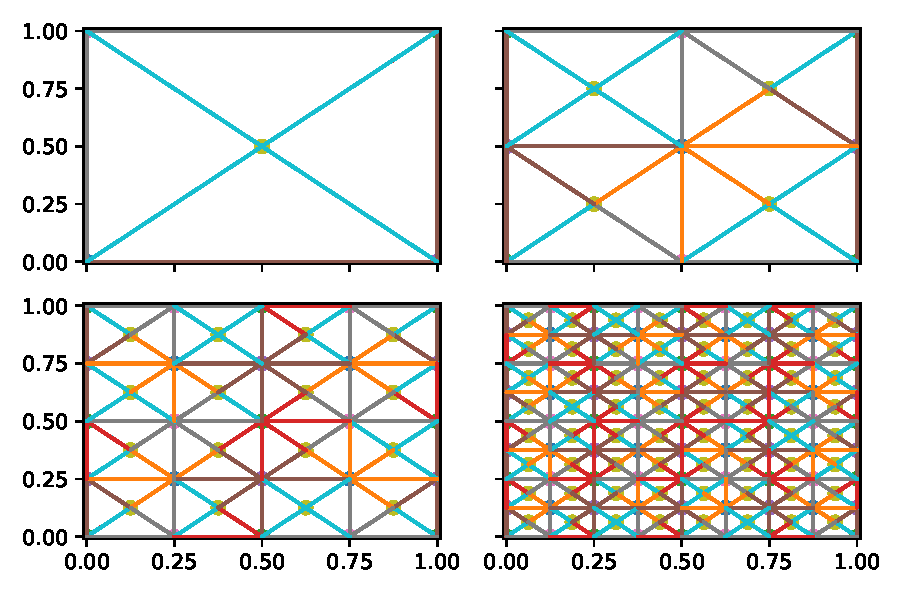
\includegraphics[scale=1.0]{./Fig10.pdf}}
{\caption{Triangulation of a unit hypercube shown in 2 dimensions for 4 iterations  \label{fig:triangles} }}
\end{figure}

In this publication we will use both the Sobol and the hypercube triangulation sampling sequences. Sobol provides a more direct comparison to the TGO algorithm while the second sequence is more similar to the DISIMPL-v algorithm. We will refer to the different uses of sampling sequences as SHGO-Sobol and SHGO-Simpl in the experimental results in \Cref{sec:results}.

\section{Theoretical comparison to the DISIMPL algorithm}
The DISIMPL algorithm developed by \citeauthor{Paul2014b} \cite{Paul2014b, paulavivcius2014simplicial, Paul2014a} is based on spatial partitioning of the search space. DISIMPL-v in particular should have a similar initial complex as SHGO-Simpl for box problems since this algorithm samples on the vertices of the simplicial complex (while DISIMPL-c samples at the geometric centre of the simplices which is more appropriate for higher dimensional problems). The graph structure of DISIMPL-v can thus be used to construct the directed complex $\mathcal{H}$ and the homological properties can be calculated and applied. An example of one such application is given in the following paragraph.

At every iteration of the DISIMPL algorithm potentially optimal simplices are selected for refinement by considerations the Lipschitz properties of the optimisation problem. In general a combination of promising simplices with good function evaluations (related to local exploration of the search space) and simplices with larger hypervolumes (related to global exploration of the search space). Gb-DISIMPL \cite{Paul2014a} is a very promising acceleration technique accomplished by switching between a "global phase" and a "usual phase". The global phase is focused on exploring simplices with larger hyper volumes and excludes smaller simplices which are potentially optimal in the usual phase. This technique prevents excessive evaluations near local minima as demonstrated in \cite{Paul2014a}. Local minima can put a "drag" on the progress of refining the minimum because the algorithm selects many neighbouring simplices that are slightly worse on the function values, but also slightly larger in volume. A meta-parameter is used in Gb-DISIMPL to select the simplices to be excluded in the global phase and was shown in \cite{Paul2014a} to be very efficient. However, using knowledge from the directed complex of $\mathcal{H}$, the domain containing these simplices near the local minima could also be identified more explicitly through a Sperner labelling if the function is known to be Lipschitz smooth.

%!!TODO: Also show the proof of the inherent lower limit of maintaining mod 2 information relating the vertices in higher dimensions (~ 10 lines) (NEXT PAPER)

%!!TODO: Mentiond the 3 triangulation schemes of the n-cube ($D_3$ etc.)

%!!TODO: Use subplots for these

%\begin{figure} \label{fig:3dg0}
%\centerline{\includegraphics[scale=0.65]{../6shgo/img/3dgen1.pdf}}
%{\caption{The initial triangulation of the 3-cube generated from the symmetry group $S_3$}}
%\end{figure}

%\begin{figure} \label{fig:3dg2}
%\centerline{\includegraphics[scale=0.65]{../6shgo/img/3dgen2.pdf}}
%{\caption{The second generation of the 3-cube generated from hyperplane cuts using the symmetry groups $S_3$ and $S_2$}}
%\end{figure}

%\begin{figure} \label{fig:3dg10}
%\centerline{\includegraphics[scale=0.65]{../6shgo/img/3dgen10.pdf}}
%{\caption{The tenth generation of the 3-cube generated from hyperplane cuts using the symmetry groups $S_3$ and $S_2$}}
%\end{figure}

%\begin{figure} \label{fig:2dg1}
%\centerline{\includegraphics[scale=0.65]{../6shgo/img/2dgen1.pdf}}
%{\caption{The initial triangulation of the 2-cube generated from the symmetry group $S_2$}}
%\end{figure}

%\begin{figure} \label{fig:2dg2}
%\centerline{\includegraphics[scale=0.65]{../6shgo/img/2dgen2.pdf}}
%{\caption{The second generation of the 2-cube generated from hyperplane cuts using the symmetry groups $S_2$ and $S_1$}}
%\end{figure}

%\begin{figure} \label{fig:3dg10}
%\centerline{\includegraphics[scale=0.65]{../6shgo/img/2dgen10.pdf}}
%{\caption{The tenth generation of the 2-cube generated from hyperplane cuts using the symmetry groups $S_2$ and $S_1$}}
%\end{figure}

%\section{Properties of complex and invariance theorem}
%\section{Homomorphisms to mod 2 homology groups}
%(For function characterisation)



\section{Algorithm implementation}
We consider two modes for the SHGO algorithm. In the first a finite number of sampling points $N$ are specified and sampling is continued until an $\Omega$ set of cardinality $N$ is produced and no further sampling occurs. This method is demonstrated by Algorithm \ref{alg:shgo1}. The main reason for this algorithm is to present a more direct comparison to TGO that can be used in numerical experiments.% we will use Algorithm \ref{alg:shgo1} in the numerical experiments.

For the purposes of global optimisation and local minima exploration Algorithm \ref{alg:shgo2} is more appropriate. By continuously calculating the $\bold{H}_1 (\mathcal{H})$ homology group several termination criteria can be used to end the sampling. For example if the amount of local minima is known the sampling can be terminated once $|\mathcal{M}|$ is large enough. Another example with many possible heuristics is tracking the historical difference in $|\mathcal{M}|$ over $|\mathcal{P}|$ and terminating sampling if $|\mathcal{M}|$ is unchanged after a certain increase in $|\mathcal{P}|$. In optimisation problems where the global minimum is known we can also use the stopping criteria such as the one defined by \cite{Paul2016} . 

\[ pe = 100\% \times \begin{cases} 
       \frac{\min\{\mathcal{F}\} - f^*}{|f^*|}, & f* \neq 0 \\
       \min\{\mathcal{F}\},  & f^* = 0
   \end{cases}
\]

Here $\min\{\mathcal{F}\}$ is the minimum function evaluation obtained including values obtained in the output of the local minimisation step as shown in the algorithm. Whatever termination criterion is used it requires an input $\bold{H}_1 (\mathcal{H})$ or $\min\{\mathcal{F}\}$ and should output a Boolean, we will refer to this function as $\mathbf{TERM}(\bold{H}_1 (\mathcal{H}), \min\{\mathcal{F}\})$ in Algorithm \ref{alg:shgo2}. In the practical implementation of the algorithm the user can also specify a finite number of iterations and/or sampling points. This functionality has been programmed into the $\mathbf{TERM}(\bold{H}_1 (\mathcal{H}), \min\{\mathcal{F}\})$ function.


Open source python implementations of both of these algorithms are available and were published under a MIT compatible license \cite{SHGOpy}.

\begin{algorithm} 
\caption{SHGO finite sampling algorithm}
\label{alg:shgo1}
\begin{algorithmic}[1]
\Procedure{Initialisation}{}
\State \bf{Input} \normalfont an objective function $f$, constraint functions $\mathbf{g}$ and variable bounds and $[\mathbf{l}, \mathbf{u}]^n$.
\State \bf{Input} \normalfont $N$ initial sampling points.
\State Define a sampling sequence that generates a set $\mathcal{X}$ of sampling points in the unit hypercube space $[\mathbf{0}, \mathbf{1}]^n$
\EndProcedure
\Procedure{Initial sampling}{}
\State $\mathcal{P} = \emptyset$
\While{$|\mathcal{P}|$ $<$ $N$}
\State Generate $N - |\mathcal{P}|$ sequential sampling points $\mathcal{X} \subset \mathbb{R}^n$
\State Stretch $\mathcal{X}$ over the lower and upper bounds $[\mathbf{l}, \mathbf{u}]^n$
\State  $\mathcal{P} = \{\mathcal{X}_i ~|~ \mathbf{g}(\mathcal{X}_i) \geq 0, \forall \mathcal{X}_i \in \mathcal{X}\} \cup\mathcal{P}$ 
\Comment (Find $\mathcal{P}$ in the feasible subset $\Omega$ by discarding any points mapped outside the linear constraints $g$ and adding to the current set of $\mathcal{P}$.)
\State Set $\mathcal{X} = \emptyset$
\EndWhile
\State Find $\mathcal{F}$ from the objective function $f: \mathcal{P} \rightarrow \mathcal{F}$
\EndProcedure
\Procedure{Construct directed complex $\mathcal{H}$}{}
\State Calculate $\mathcal{H}$ from $h: \mathcal{P}\rightarrow \mathcal{H}$
\EndProcedure
\Procedure{Construct $\mathcal{M}$}{}
\State Find $\mathcal{M}$ from \Cref{def:h4}.
\EndProcedure
\Procedure{Local minimisation}{}
\State Calculate the approximate local minima of $f$ using a local minimisation routine with the elements of $\mathcal{M}$ as starting points.
\Comment These local minimisations can be performed in parallel.
\EndProcedure
\Procedure{Process return objects}{}
\State Order the final outputs of the minima of $f$ found in the local minimisation step to find the approximate global minimum.
\EndProcedure \\
\Return the approximate global minimum and a list of all the minima found in the local minimisation step.
\end{algorithmic}
\end{algorithm} 





\begin{algorithm} 
\caption{SHGO homology group growth algorithm}
\label{alg:shgo2}
\begin{algorithmic}[1]
\Procedure{Initialisation}{}
\State \bf{Input} \normalfont an objective function $f$, constraint functions $\mathbf{g}$ and variable bounds and $[\mathbf{l}, \mathbf{u}]^n$.
\State \bf{Input} \normalfont $N$ initial sampling points.
\State Define a sampling sequence that generates a set $\mathcal{X}$ of sampling points in the unit hypercube space $[\mathbf{0}, \mathbf{1}]^n$
\State Define the empty set $\mathcal{M}^E = \emptyset$ of vertices evaluated by a local minimisation.
\EndProcedure
\While{$\mathbf{TERM}(\bold{H}_1 (\mathcal{H}), \min\{\mathcal{F}\})$ is False}
\Procedure{Sampling}{}
\State $\mathcal{P} = \emptyset$
\While{$|\mathcal{P}|$ $<$ $N$}
\State Generate $N - |\mathcal{P}|$ sequential sampling points $\mathcal{X} \subset \mathbb{R}^n$
\State Stretch $\mathcal{X}$ over the lower and upper bounds $[\mathbf{l}, \mathbf{u}]^n$
\State  $\mathcal{P} = \{\mathcal{X}_i ~|~ \mathbf{g}(\mathcal{X}_i)  \geq 0, \forall \mathcal{X}_i \in \mathcal{X}\} \cup\mathcal{P}$ 
\Comment (Find $\mathcal{P}$ in the feasible subset $\Omega$ by discarding any points mapped outside the linear constraints $g$ and adding to the current set of $\mathcal{P}$.)
\State Set $\mathcal{X} = \emptyset$
\EndWhile
\State Find $\mathcal{F}$ from the objective function $f: \mathcal{P} \rightarrow \mathcal{F}$ for any new points in $\mathcal{P}$
\EndProcedure
\Procedure{Construct/append  directed complex $\mathcal{H}$}{}
\State Calculate $\mathcal{H}$ from $h: \mathcal{P}\rightarrow \mathcal{H}$  
\Comment (If $\mathcal{H}$ was already constructed new points in $\mathcal{P}$ are incorporated into the triangulation.)
\State Calculate $\bold{H}_1 (\mathcal{H})$
\EndProcedure
\Procedure{Construct $\mathcal{M}$}{}
\State Find $\mathcal{M}$ from \Cref{def:h4}.
\EndProcedure
\Procedure{Local minimisation}{}
\State Calculate the approximate local minima of $f$ using a local minimisation routine with the elements of $\mathcal{M} \setminus \mathcal{M}^E$ as starting points. 
\Comment Process the most promising points first.
\State $\mathcal{M}^E = \mathcal{M}^E \cap \mathcal{M}$  \Comment This excludes the evaluation any element $ v_i \in \mathcal{M}$ that is known to be the only point that in the domain $\partial \textrm{st}(v_j)$ where $v_j$ is known to any point already used as a starting point in Step 27. If any new $ v_i \in \mathcal{M}$ not in $\mathcal{M}^E $ is known to be the only point $\partial \textrm{st}(v_j)$ it can also be excluded.
\State Add the function outputs of the local minimisation routine to $\mathcal{F}$
\EndProcedure
\State Find new value of $\mathbf{TERM}(\bold{H}_1) (\mathcal{H}, \min\{\mathcal{F}\})$
\EndWhile
\Procedure{Process return objects}{}
\State Order the final outputs of the minima of $f$ found in the local minimisation step to find the approximate global minimum.
\EndProcedure \\
\Return the approximate global minimum and a list of all the minima found in the local minimisation step.
\end{algorithmic}
\end{algorithm} 

